\documentclass[times, utf8, diplomski,  numeric]{fer}
\usepackage{booktabs}
\usepackage{pdfpages}
\graphicspath{ {./images/} }

\usepackage{listings}
\usepackage{color}
\usepackage[hidelinks]{hyperref}
\usepackage{mathrsfs}
\usepackage{float}
\usepackage{amsmath,amssymb}
\usepackage{subcaption}

\definecolor{codegreen}{rgb}{0,0.5,0}
\definecolor{codegray}{rgb}{0.5,0.5,0.5}
\definecolor{codered}{rgb}{0.82,0,0.25}
\definecolor{codeorange}{rgb}{1,0.5,0.25}
\definecolor{backcolour}{rgb}{0.95,0.95,0.92}
 
\lstdefinestyle{mystyle}{
   basicstyle=\ttfamily,
    backgroundcolor=\color{backcolour},   
    commentstyle=\color{codegreen},
    keywordstyle=\color{codeorange},
    numberstyle=\tiny\color{codegray},
    stringstyle=\color{codered},
    basicstyle=\footnotesize,
    breakatwhitespace=false,         
    breaklines=true,                 
    captionpos=b,                    
    keepspaces=true,                 
    numbers=left,                    
    numbersep=5pt,                  
    showspaces=false,                
    showstringspaces=false,
    showtabs=false,                  
    tabsize=2
}
 

\lstset{style=mystyle}

\begin{document}

% TODO: Navedite broj rada.
\thesisnumber{2095}

% TODO: Navedite naslov rada.
\title{Konvolucijski modeli za klasifikaciju videa}

% TODO: Navedite vaše ime i prezime.
\author{Antonio Borac}

\maketitle

% Ispis stranice s napomenom o umetanju izvornika rada. Uklonite naredbu \izvornik ako želite izbaciti tu stranicu.
%\izvornik
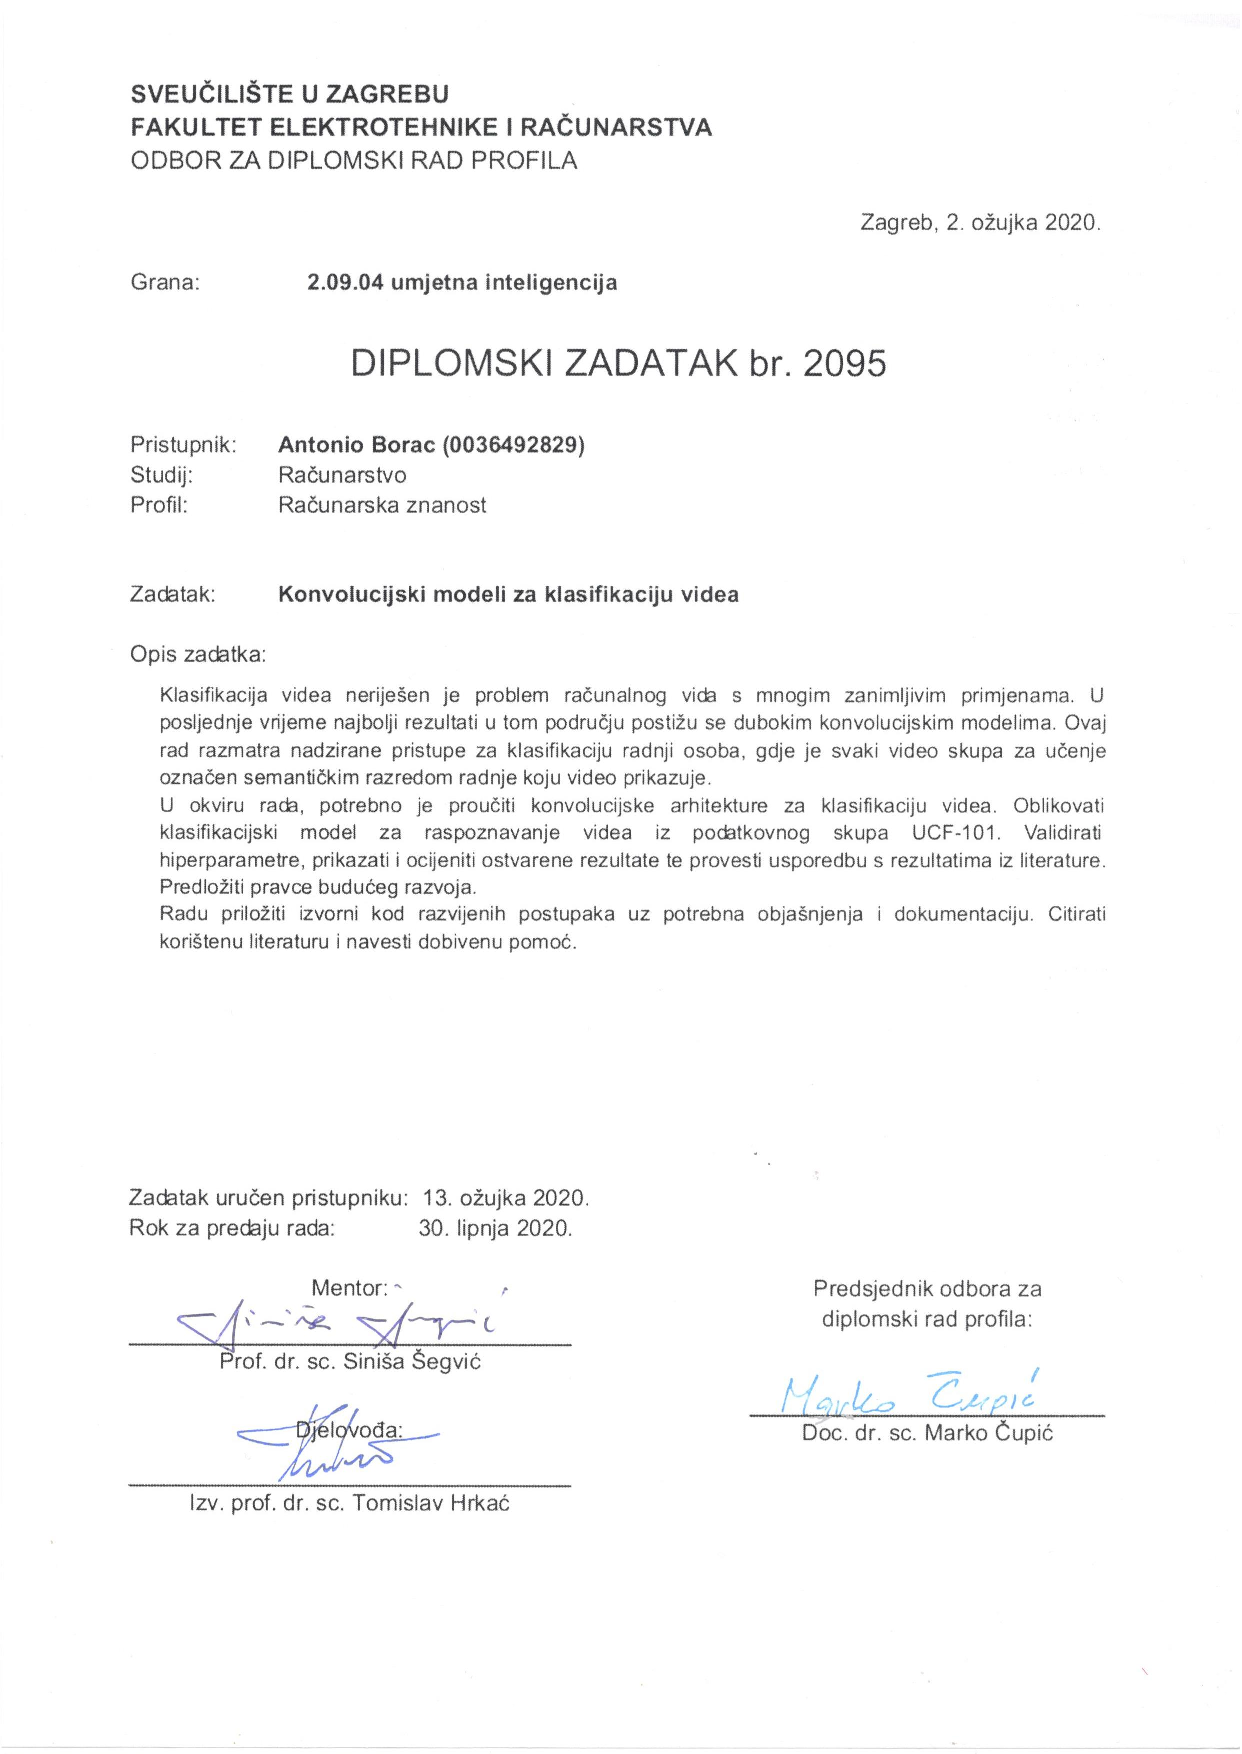
\includepdf{izvornik.pdf}

% Dodavanje zahvale ili prazne stranice. Ako ne želite dodati zahvalu, naredbu ostavite radi prazne stranice.
\zahvala{Zahvaljujem mentoru prof. dr. sc. Siniši Šegvicu na pruženoj pomoći tijekom studiranja i pri izradi ovog rada. Hvala mojoj obitelji i prijateljima na strpljenju i podršci tijekom cijelog školovanja.}

\tableofcontents

\chapter{Uvod}
Duboko učenje je od svojih početaka znatno napredovalo. Za takav napredak su najviše zaslužni intenzivni razvoj sklopovlja koji podržava izrazito paralelnu obradu podataka i razvoj algoritama koji efikasno koriste takvo sklopovlje. U posljednjih nekoliko godina izgrađeni su brojni modeli koji uspješno rješavaju problem klasifikacije slika, na kojem postižu bolje rezultate od čovjeka. U istraživanjima su uglavnom zastupljeni modeli koji se koriste za klasifikaciju slika, prepoznavanje govora i analizu teksta. Uspjesi postignuti na tim problemima naveli su stručnjake da pokušaju riješiti složenije probleme poput klasifikacije videa metodama dubokog učenja. 
\par
Klasifikacija videa neriješen je problem računalnog vida s mnogim zanimljivim primjenama. Iako je video niz od $N$ sličica odnosno okvira, klasifikacija videa nije samo klasifikacija $N$ sličica. Prilikom klasifikacije videa u obzir se mora uzeti i odnos između pojedinih okvira videa. Obično pretpostavljamo da su susjedni okviri u videu korelirani i modeli za klasifikaciju videa moraju uzeti tu činjenicu u obzir. U posljednje vrijeme najbolji rezultati u području klasifikacije videa postižu se dubokim konvolucijskim modelima. Prije nego što su se masovno počeli koristiti konvolucijski modeli, istraživanja na području klasifikacije videa su vodila u smjeru histograma slikovnih riječi, te su se za samu klasifikaciju često koristili SVM modeli \cite{6909619}. 
\par
U okviru rada ćemo objasniti česte pojmove u području dubokog učenja i opširno ćemo opisati ključne komponente nužne za razvoj dubokih modela za klasifikaciju videa. Detaljno ćemo razmotriti dvije arhitekture koje ostvaruju dobre rezultate na skupovima namijenjenima za učenje modela za klasifikaciju videa. Osim samih arhitektura, opisat ćemo i kralježničke modele \engl{backbone} koje koristimo. Razmotrit ćemo kako pristupiti videu kao podatku za učenje. Izgradit ćemo opisane modele i evaluirati ostvarene rezultate.
\par
U izgradnji naših modela nam uvelike pomažu programski okviri visokog nivoa poput Kerasa \cite{Keras} i PyTorcha \cite{Pytorch}. Za izgradnju naših modela smo odlučili koristiti programski okvir Keras. U okviru rada ćemo dati kratak pregled navedenog programskog okvira i prikazat ćemo kako jednostavno i brzo izgraditi željene modele.
\par
Iz naših eksperimenata ćemo izvesti zaključak u kojem ćemo sažeto iznijeti postignute rezultate. Usporedit ćemo dobivene rezultate s rezultatima iz literature i dati prijedloge za eventualno poboljšanje. Navest ćemo prijedloge za daljnji rad temeljen na izvedenim eksperimentima u sklopu ovog rada.

\chapter{Duboko učenje}
U ovom poglavlju ćemo se upoznati sa ključnim slojevima na kojima se baziraju naši modeli. Razumijevanje načina rada tih slojeva je veoma važno za razumijevanje arhitektura koje razmatramo u okviru našeg rada.
\par
Za početak, upoznajmo se sa osnovnim pojmovima dubokog učenja.
\subsubsection{Aktivacijska funkcija}
Kako bi konvolucijskim modelima mogli modelirati nelinearne funkcije, možemo koristiti različite nelinearne aktivacijske funkcije. Najpoznatije aktivacijske funkcije koje se koriste su linearna aktivacijska funkcija, softmax funkcija, sigmoidalna funkcija i funkcija zglobnice.
\par
Linearna aktivacijska funkcija je definirana formulom $h(x)=x$.
\begin{figure}[htb]
\centering
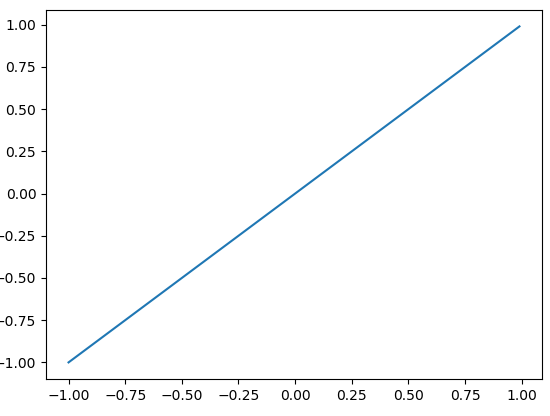
\includegraphics[width=8cm]{./images/linear}
\caption{Linearna aktivacijska funkcija.}
\label{fig:linear}
\end{figure}
\par
Funkcija zglobnica \engl{rectified linear unit, ReLU} je definirana formulom $h(x)=max(0,x)$. Uz popularnu ReLU funkciju, primjenu nalazi i propusna zglobnica \engl{Leaky ReLU} koja je definirana formulom $h(x)=max(\alpha x,x), \alpha\geq 0$. Propusna zglobnica je pokušaj rješavanja problema umiruće zglobnice \engl{dying ReLU} koji se pojavljuje kod funkcije zglobnice kad se u modelu ne koristi sloj normalizacije po grupama. Problem kod zglobnice je što joj je derivacija jednaka 0 za $x < 0$. U tom slučaju dolazi do potencijalno neželjenog gašenja neurona.

\begin{figure}[htp]

\centering
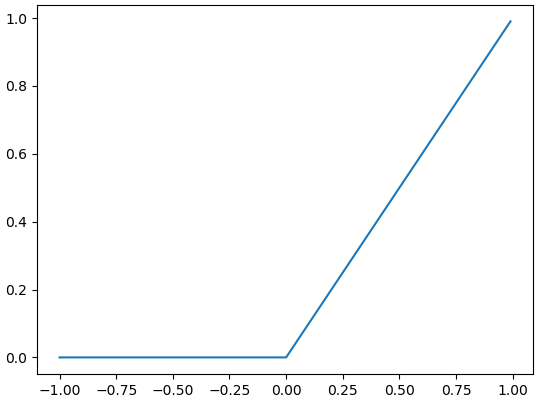
\includegraphics[width=.5\textwidth]{./images/relu}\hfill
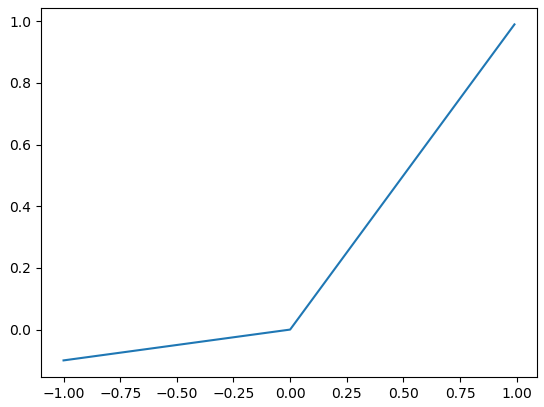
\includegraphics[width=.5\textwidth]{./images/lrelu}

\caption{ReLU(lijevo) i LeakyReLU(desno).}
\label{fig:relu}
\end{figure}
\par
Sigmoidalna funkcija je definirana formulom $h(x)=\frac{1}{1+\exp^{-x}}$. Prednost sigmoidalne aktivacijske funkcije je što joj je kodomena skup $<0,1>$, pa se može interpretirati kao vjerojatnost. Sigmoida ima neželjeno svojstvo - za velike pozitivne i negativne vrijednosti ulazi u područje zasićenja. Gradijent funkcije u tom području postaje malen i neuron više ne može učiti. Taj problem u literaturi nazivamo problemom nestajućih gradijenata. Upravo taj problem je jedan od problema koji su ograničavali duboke modele. Problem je umanjen korištenjem aktivacijske funkcije zglobnice i sloja normalizacije po grupama.
\begin{figure}[htp]

\centering
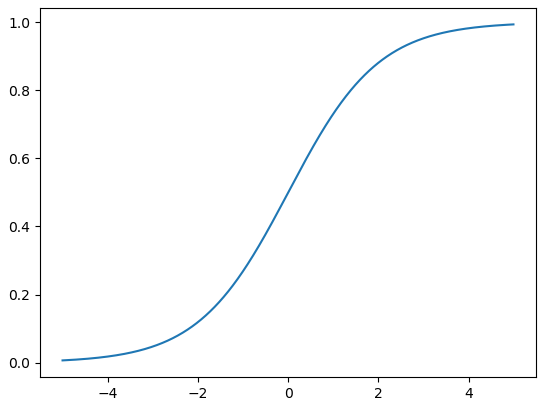
\includegraphics[width=8cm]{./images/sigmoid}\hfill

\caption{Sigmoidalna aktivacijska funkcija.}
\label{fig:sigmoid}
\end{figure}
\par
Funkcija softmax je definirana formulom $h(x)_i=\frac{\exp(z_i)}{\sum_{j=1}^K \exp(z_j)}$ za $i = 1,...,K$ i $z=(z_1,...,z_k) \in R^K$. Možemo primjetiti da je $h(x)_i$ vrijednost u skupu $<0,1>$ i da je $\sum_{i}^{K} h(x)_i$ jednaka 1, pa vrijednost $h(x)_i$ možemo intepretirati kao vjerojatnost pripadnosti $x$ $i$-tom razredu.
\par
Primjena aktivacijske funkcije zglobnice na aktivacije skrivenih slojeva je jedan od ključnih faktora koji je omogućio uspješno učenje dubokih modela. 
\subsubsection{Funkcija gubitka}
Funkcija gubitka predstavlja mjeru troška nekog događaja. U kontekstu dubokog učenja predstavlja mjeru odstupanja stvarnog izlaza modela od željenog izlaza za dani ulaz. Cilj učenja modela je smanjiti vrijednost funkcije gubitka za dane ulaze, odnosno optimizirati funkciju gubitka. Postoje brojne funkcije gubitka koje se koriste u dubokom učenju ovisno o problemu koji se rješava. Tako u regresijskim modelima često susrećemo srednju kvadratnu pogrešku \engl{Mean Absolute Error}, dok u klasifikacijskim problemima često susrećemo unakrsnu entropiju \engl{Cross Entropy Loss}, funkciju koju ćemo i mi optimizirati u našim eksperimentima. Tu pogrešku računamo na sljedeći način: 
\begin{equation}
L_{i} = - \sum_{j}^{K} y_{i,j} \log{p_{i,j}} 
\end{equation}
gdje je \verb|K| broj razreda, $y_{i,j}$ 1 ako $i$-ti primjer pripada $j$-tom razredu inače 0, $p_{i,j}$ vjerojatnost pripadnosti $i$-tog primjera $j$-tom razredu. $p_{i,j}$ je izlaz \verb|softmaks| funkcije, a $y_{i}$ je jedinični vektor koji ima vrijednost $1$ na indeksu razreda kojem primjer pripada, pod uvjetom da su razredi poredani.
\subsubsection{Optimizacijski postupak}
Optimizacijskim postupkom nastojimo korigirati parametre neuronskih mreža kako bi mreža predstavljala što bolju aproksimaciju funkcije koju želimo modelirati. Naime, za razliku od klasičnog optimizacijskog problema kod kojih je poznata distribucija koju modeliramo, u dubokom učenju to najčešće nije slučaj. Optimiramo neku mjeru gubitka J u nadi da ćemo indirektno optimirati i originalnu mjeru P. Taj postupak je najčešće iterativan. Česti optimizacijski postupci koje koristimo su Adam, stohastički gradijentni spust i Adagrad. Postoji mnogo optimizacijskih postupaka koji se koriste ovisno o problemu koji se rješava.
\par
Stohastički gradijentni spust je iterativna metoda za optimizaciju funkcije. Ideja koja se krije iza ove metode je da za informaciju o daljnjem smjeru u kojem trebamo ići sa parametrima funkcije koristimo gradijent funkcije. Prva derivacija derivabilne funkcije pokazuje smjer najbržeg porasta vrijednosti funkcije gubitka. Želimo se kretati u smjeru suprotnom od smjera najvećeg porasta kako bi smanjili vrijednost funkcije gubitka u sljedećoj iteraciji. Bitno je istaknuti da se samo ažuriranje težina može obaviti nakon svakog primjera koje model vidi, nakon nekoliko primjera i nakon svih primjera skupa za treniranje. Ako ažuriranje obavljamo nakon svakog primjera, govorimo o online učenju, pri čemu je gradijent samo aproksimacija pravog gradijenta. Tada je formula za stohastički gradijentni spust 
\begin{equation}
w = w - \eta \nabla f(x_{i})
\end{equation}
 gdje je $w$  težina koju ažuriramo, $\eta$ stopa učenja. Kad ažuriranje obavljamo nakon svih primjera, govorimo o offline učenju, te formula tada postaje
\begin{equation}
w = w - \eta \sum_{i=0}^{N} \nabla f(x_{i})
\end{equation}  gdje je $N$ broj primjera u skupu za učenje. U tom slučaju govorimo o učenju s grupama. Kad ažuriranje obavljamo nakon nekoliko primjera, govorimo o učenju s mini grupama. U slučaju kad za učenje koristimo cijeli skup za treniranje, gradijent u lokalnim i globalnim optimuma funkcije gubitka iznosi 0, dok u slučaju kad koristimo manje primjera to ne mora biti slučaj.
\par
Optimizacijski postupak Adam je također iterativan postupak kao i stohastički gradijentni spust. Pripada grupi algoritama koji koriste moment za učenje modela. Algoritam prati eksponcijalni pomični prosjek gradijenata i kvadrata gradijenata. Korekcija se obavlja prema eksponencijalnom pomičnom prosjeku gradijenata a ne prema izračunatom gradijentu u određenom koraku.
\subsubsection{Regularizacija}
Prilikom optimizacije funkcije gubitka, često dolazi do problema da model previše dobro nauči klasificirati uzorke iz skupa za učenje, odnosno da "nauči napamet" skup za učenje. Model tad ne modelira željenu funkciju već se ponaša kao memorija koja pamti podatke iz skupa za učenje. Ako na ulaz modela dovedemo neki uzorak koji model do tad nije vidio, model će se loše ponašati. Taj problem želimo ublažiti brojnim tehnikama regularizacije. U sklopu naših eksperimenata, između ostalog koristimo L2 regularizaciju, sloj normalizacije po grupama i povećanje skupa podataka za učenje. L2 regularizacija na funkciju gubitka modela dodaje regularizacijski faktor koji ovisi o normi vektora težina.
\newpage
\section{Konvolucijski modeli}
Konvolucijske neuronske mreže su specijalizacija modela sa potpuno povezanim slojevima. Za razliku od modela s potpuno povezanim slojevima, koriste konvolucijske slojeve u skrivenim slojevima mreže. Konvolucijski slojevi modeliraju lokalnu interakciju i dijele parametre, što im omogućava korištenje manje parametara u odnosu na  modele s potpuno povezanim slojevima \cite{du-web}. Pokazali su se kao dobar pristup širokom spektru problema računalnog vida. Danas, većina od modela koji ostvaruju najbolje rezultate na skupovima za klasifikaciju slika su upravo konvolucijski modeli \cite{leaderboards}. U nastavku ćemo opisati te slojeve, kako ti slojevi rade te za što se koriste.
\subsection{Konvolucijski sloj}
Konvolucijski slojevi predstavljaju najvažnije slojeve u konvolucijskim modelima. Naziv su dobili po operaciji konvolucije\footnote{U strojnom učenju pod operaciju konvolucije podrazumijevamo operaciju unakrnse korelacije \cite{du-web}.} koju provode nad ulaznim podacima. Sama operacija je diferencijabilna, što ju čini iznimno privlačnom za korištenje u modelima koji su optimizirani sa algoritmima učenja koji koriste gradijente. 
\par
Operacija konvolucije se provodi uz pomoć filtra. Filtar je matrica težina kojom se množe pripadajući dijelovi ulazne mape značajki kako bi se dobio element izlazne mape značajki. Princip rada filtra je dobro prikazan na slici \ref{fig:convolution}. Svaki konvolucijski sloj sadrži filtar kojim se obavlja operacija konvolucije. Operaciju je najjednostavnije objasniti na jednom primjeru. Ulaz u sloj je slika dimenzija \verb|32x32x3|. Koristimo filtar sa 16 filtra dimenzija \verb|3x3|. Jezgru po ulazu pomičemo za 1 u horizontalnom i vertikalnom smjeru. Filtar operaciju konvolucije provodi nad svim kanalima ulazne mape značajki, tako da je zapravo dimenzija svakog filtra \verb|3x3x3|. Dubina izlazne mape značajki će biti jednaka broju filtara koji koristimo, što je u našem slučaju jednako 16. Prostorne dimenzije izlaznog sloja računamo pomoću sljedeće formule: $W_{out} = (W_{in} - F + 2P) / S + 1$, gdje je $W_{in}$ prostorna dimenzija ulaza, $F$ dimenzija jezgre, $P$ broj nula koje nadodajemo oko podataka po dimenziji koju računamo što je bitno za dimenzije izlazne mape značajki, $S$ pomak po ulazu a $W_{out}$ prostorna dimenzija izlaza. Prema toj formuli, primjerice širina izlazne mape značajki u našem slučaju postaje $W_{out} = (32 - 3 + 2*0) / 1 + 1 = 30$. Dimenzija izlazne mape značajki je \verb|30x30x16|. Primjetimo da smo u ovom slučaju izabrali $P$ jednak 0, odnosno ne koristimo nadopunjavanje ulazne mape značajki, što je dovelo do smanjenja prostornih dimenzija izlazne mape značajki. U literaturi, takva postavka nadopunjavanja je često nazvana "valid". Često se koristi i nadopunjavanje nulama koje bi dovelo do toga da prostorne dimenzije izlazne mape značajki ostanu jednake prostornim dimenzijama ulazne mape značajki. U literaturi, takvu postavku nadopunjavanja često zovemo "same".  
\begin{figure}[htp]

\centering
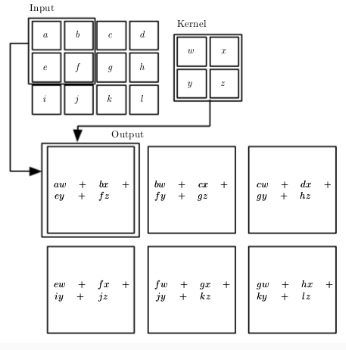
\includegraphics[width=8cm]{./images/du-convolution}\hfill

\caption{Prikaz operacije konvolucije. Slika je preuzeta iz \cite{Goodfellow-et-al-2016}.}
\label{fig:convolution}
Na slici ~\ref{fig:convolution} možemo vidjeti kako se odvija operacija konvolucije. Jezgru filtra pomičemo po ulaznoj mapi značajki. Svaki element prozora ulazne mape značajki množimo sa poklapajućim elementom jezgre. Dobivene brojeve zbrojimo i pomičemo jezgru za pomak \verb|s| kako bi izračunali sljedeći element izlazne mape značajki.
\end{figure} 
\subsection{Potpuno povezani sloj}
U potpuno povezanom sloju je svaka aktivacija prethodnog sloja povezana sa svakim neuronom trenutnog sloja. Ako broj aktivacija u prethodnom sloju označimo sa \verb|n|, izlaz j-tog neurona potpuno povezanog sloja tada je:
\begin{equation}
x_{j} = \sum_{i}^{n} x_{i,j-1} w_{i,j-1} + b_{j} 
\end{equation},
gdje je $b_{j}$ prag za j-ti neuron. Vidljivo je da je na ovaj način moguće modelirati samo linearne funkcije, pa često na izlaz neurona dodajemo neku nelinearnu funkciju koju nazivamo aktivacijska funkcija. Tada izlaz j-tog neurona uz nelinearnu aktivacijsku funkciju $\rho$ postaje:
\begin{equation}
x_{j} = \rho(\sum_{i}^{n} x_{i,j-1} w_{i,j-1} + b_{j}) 
\end{equation}.
Ako je \verb|n| broj izlaza prethodnog sloja, a \verb|m| broj neurona u trenutnom sloju i ako uzmemo u obzir sve pragove za svaki neuron, tada će potpuno povezani sloj ukupno imati \verb|m*n+m| težina.
\par
U konvolucijskim modelima potpuno povezane slojeve često susrećemo "na kraju" modela, gdje se koristi sa aktivacijskom funkcijom softmaks kako bi izlaz modela dao vjerojatnost klasifikacije ulaznog podatka za svaki semantički razred skupa podataka. Izbjegavamo ih koristiti u početnim dijelovima konvolucijskog modela jer unose jako puno parametara.
\subsection{Sloj sažimanja}
Sloj sažimanja najčešće se koristilo kako bi se smanjile prostorne dimenzije ulazne mape značajki što je vodilo do smanjenja broja parametara i utjecalo na smanjivanje pretreniranosti modela. Danas se sloj sažimanja koristi za smanjenje memorijskog i računskog opterećenja prilikom učenja i evaluiranja modela.
\par
 Svaki sloj sažimanja ima definiran prozor sažimanja koji provodi definiranu operaciju nad dijelom ulazne mape značajki. Postoji niz operacija koje je moguće provoditi nad prozorom ulazne mape značajki, od kojih najčešće susrećemo operaciju maksimuma i aritmetičke sredine. Sloj sažimanja maksimumom kao rezultat daje maksimum iz trenutnog prozora iz ulazne mape značajki. Bitno je napomenuti da dubina izlazne mape značajki ostaje ista dubini ulazne mape značajki, što nije nužno bio slučaj kod konvolucijskog sloja gdje je dubina izlazne mape značajki jednaka broju jezgri. Širinu izlazne mape značajki računamo pomoću sljedeće formule: \( w_{out}=(w_{in}-p)/s+1\), gdje je $p$ širina prozora sažimanja, $w_{in}$ širina ulazne mape značajki, $s$ pomak prozora po širini. Analogno računamo i visinu izlazne mape značajki.
\par
U praksi u konvolucijskim modelima često surećemo slojeve globalnog sažimanja. Obično ih susrećemo na kraju konvolucijskog modela gdje je dubina mape značajki veća od širine i visine. Efektivno, prozor kod globalnog sažimanja je jednak prostornim dimenzijama mape značajki, što znači da je izlaz ovog sloja jednak \verb|1x1xD|, gdje je  $D$ dubina mape značajki.
\subsection{Normalizacija po grupama}
Normalizacija po grupama \engl{batch normalization} je široko rasprostranjena tehnika koja omogućava brže i stabilnije treniranje dubokih modela \cite{NIPS2018_7515}. Tehnika radi tako da stabilizira distribuciju ulaza sloja koju kontroliraju srednja vrijednost i varijanca ulaza. Kod dubokih modela, istoremena korekcija težina u svim slojevima stvara problem jer su slojevi povezani - izlaz jednog sloja predstavlja ulaz drugog sloja. Dolazi do efekta promjene ulaznih podataka za drugi sloj što se naziva kovarijacijski pomak. To želimo izbjeći, izlaz svakog sloja bi trebao ponovno biti normaliziran što sljedećem sloju osigurava stabilnije ulaze. Normalizacija se radi na temelju izlaza koje taj neuron ima kad na ulaz mreže dovedemo sve primjere iz mini grupe \cite{du-web}. Računa se srednja vrijednost odziva neurona i varijanca na temelju ulaznih podataka. Pomoću tih vrijednosti normaliziramo odziv za svaki ulaz iz mini grupe, skaliramo izlaz i dodajemo pomak. Formula koja prikazuje taj postupak je $y = \alpha y' + \beta $, gdje je $y'$ normalizirani izlaz, $y$ konačni izlaz, $\alpha$ parametar za skaliranje i $\beta$ fiksni pomak. Parametri $\alpha$ i $\beta$ se uče tijekom faze učenja modela.
\par
Smatralo se da normalizacija po grupama efikasno pomaže pri učenju modela zato jer smanjuje interni kovarijacijski pomak. Rad \cite{NIPS2018_7515} otkirva da je najveći doprinos sloja normalizacije po grupama taj da značajno zaglađuje funkciju cilja. Takvo zaglađivanje funkcije cilja vodi do stabilnijeg ponašanja gradijenata što dalje vodi do bržeg učenja.  
\subsection{Slojevi za trodimenzionalne podatke}
Iako se najčešće susrećemo sa operacijama konvolucije i sažimanja koje koriste dvodimenzionalne prozore i jezgre, moguće je susresti i višedimenzionalne prozore i jezgre. U okviru ovog rada se susrećemo sa konvolucijskim slojevima i slojevima sažimanja koji imaju trodimenzionalnu jezgru. U tom slučaju, na ulaz primamo tenzor sljedećih dimenzija: \verb|(batch_size, sp1, sp2, temp, channels)|. U slučaju 2d konvolucijskog sloja jezgra se pomiče u horizontalnom i vertikalnom smjeru po ulaznoj mapi značajki i pri svakom pomaku kreira jedan element izlazne mape značajki. Takvim pomicanjem jezgre nastaje jedna matrica za svaku jezgru konvolucijskog sloja. U slučaju trodimenzionalnih jezgri, osim što se jezgre pomiču u horizontalnom i vertikalnom smjeru, pomiču se i po dodatnoj dimenziji. Rezultat djelovanja svake jezgre bit će po jedan volumen. Operacija koja se provodi se pri tome ne mijenja, osim što za jedan element izlazne mape značajki računamo konvoluciju trodimenzionalne jezgre sa trenutnim dijelom ulaznog volumena. Ista stvar vrijedi i za slojeve sažimanja.
\par
Ovakvi slojevi se koriste za sekvencijalne\footnote{Sekvencijanim podacima nazivamo sve podatke kod kojih je bitan poredak.} podatke kao što je video.
\chapter{Konvolucijski modeli za klasifikaciju videa}
\section{Kralježnička arhitektura \engl{backbone}}
U okviru našeg rada, "backbone" arhitekturom smatramo dio mreže koji koristimo za ekstrakciju značajki. U našim eksperimentima ćemo koristiti modele koji su predtrenirani na Imagenet skupu podataka kako bi ubrzali proces učenja cjelokupnog modela. Imagenet je skup podataka koji se koristi za klasifikaciju slika koji sadrži preko 14 milijuna podataka i koji je označen sa preko 20 000 razreda. Ako prilikom treniranja modela težine inicijaliziramo nasumičnim vrijednostima, izlazi modela na samom početku treniranja će biti slučajni. Tek nakon treniranja modela kroz određen broj epoha će težine biti postavljene na određene vrijednosti uz koje izlaz mreže ima smisla. Predtreniranje je postupak kojim ubrzavamo taj proces. Druga velika prednost predtreniranja modela je što je model moguće naučiti sa manje primjera za učenje \cite{Oquab_2014_CVPR} unatoč tome što distribucije težina na problemu na kojem se težine predtreniraju i na problemu koji se rješava nisu iste. Ako težine inicijalno postavimo na vrijednosti dobivene treniranjem na nekom bliskom problemu, modelu će vjerojatno trebati manje vremena da nauči težine koje su dobre za trenutni problem koji rješavamo od nasumične inicijalizacije.
\par
Iako predtreniranje na skupovima poput Imageneta nije nužno\footnote{Rad \cite{rethinking} pokazuje da predtreniranje nije nužno i da se jednako dobri rezultati mogu dobiti slučajnom inicijalizacijom na problemima poput detekcije ako model učimo na jako velikom skupu podataka. U slučaju kad imamo jako malo podataka za učenje, predtreniranje je ključno za postizanje dobrog rezultata \cite{orsic19cvpr}.} za dobre rezultate modela, u praksi se pokazuje da predtreniranje na Imagenetu i kasnije ugađanje na skupu nad kojim obavljamo treniranje ubrzava konvergenciju. U radu ćemo koristiti ekstraktore značajki koji su trenirani na Imagenet skupu podataka koje ćemo ugađati u nadi da ćemo dobiti dobre rezultate.
\subsection{Konvolucijski modeli sa rezidualnim vezama}
Duboki konvolucijski modeli sa rezidualnim vezama su prisutni od 2015. te su od samog predstavljanja postali jako popularni. Koriste se na gotovo svim područjima računalnog vida. Velik problem kod učenja dubokoh modela predstavljao je problem nestajućih gradijenata. Taj problem je uglavnom riješen normalizacijom ulaza i korištenjem slojeva normalizacije. Duboki modeli počinju konvergirati korištenjem navedenih slojeva, ali se uočava drugi problem - problem degradacije točnosti. Povećanjem broja slojeva modela dolazi do zasićenja točnosti, pa daljnjim povećanjem broja slojeva i do degradacije točnosti. Iako bi očekivali da do smanjenja točnosti dolazi zbog prenaučenosti, pokazuje se da to nije slučaj. Dodavanjem slojeva na model koji pokazuje dobre rezultate dolazi do povećanja pogreške na skupu za učenje. Rad \cite{resnet} problemu degradacije pristupa uvođenjem rezidualnih veza. 
\par
Ako pretpostavimo da niz slojeva može aproksimirati neku složenu funkciju $H(x)$, možemo pretpostaviti da slojevi mogu također mogu aproksimirati neku složenu funkciju $F(x) = H(x) - x$. Ako model aproksimira funkciju $F(x)$, originalna funkcija koju je potrebno modelirati postaje $F(x) + x$. Rad \cite{resnet} pretpostavlja da je takvo mapiranje lakše naučiti nego originalno mapiranje $H(x)$. Formulacija $F(x) + x$ može biti ostvarena sa unaprijednom neuronskom mrežom sa preskočnim vezama. Preskočne veze preskaču jedan ili više slojeva u modelu. U okviru rada, preskočne veze preskaču  niz od nekoliko slojeva, na izlaz niza slojeva se dodaje doprinos preskočne veze. Takvu konstrukciju nazivamo rezidualna jedinica. Preskočne veze ne unose nove parametre u model i ne povećavaju složenost. 
\par
\begin{figure}[htb]
\centering
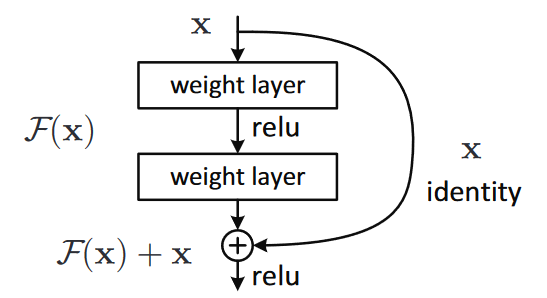
\includegraphics[width=8cm]{./images/residual_block}
\caption{Prikaz rezidualne jedinice. Prikaz je preuzet iz \cite{resnet}.}
\label{fig:resblock}
\end{figure}
Ovakav postupak ima mnogo prednosti. Osim što dodatno umanjuje problem nestajućih gradijenata, omogućava gradnju kompleksnijih ovisnosti u mreži. Omogućava direktnu propagaciju informacija kroz slojeve, odnosno omogućava učenje slojeva koji direktno ovise o "plićim" dijelovima modela.
\par
Predlažu se dva načina slaganja rezidualnih jedinica. Prvi način je osnovni način \engl{basic} gdje se u svakoj rezidualnoj jedinici koriste dva konvolucijska sloja sa jezgrom \verb|3x3|. Drugi način je usko grlo \engl{bottleneck} gdje se koriste tri konvolucijska sloja, redom \verb|1x1|, \verb|3x3| i \verb|1x1|, gdje su \verb|1x1| slojevi zaduženi za smanjivanje i potom povećavanje dimenzija kako bi \verb|3x3| sloj imao manje ulazne i izlazne dimenzije. Drugi način se koristi u dubljim rezidualnim arhitekturama kako bi se kontrolirao broj parametara. Nakon svakog konvolucijskog sloja dolazi sloj normalizacije po grupi i zglobnica kako bi se smanjio utjecaj nestajućih gradijenata.
\par
Na arhitekturi se kontinuirano radi uz mnoga poboljšanja. Poznato je da neke arhitekture u praksi pokazuju dobre rezultate ali nam nije odmah jasno zašto. Jedna od takvih arhitektura je i rezidualna arhitektura. Preskočne veze zaglađuju funkciju cilja što pomaže pri učenju modela.
\begin{figure}[htb]
\begin{subfigure}[t]{.5\textwidth}
\centering
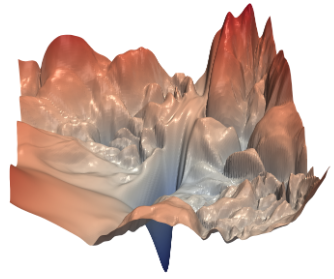
\includegraphics[width=8cm]{./images/loss-noshort}
\caption{}
\label{fig:resloss1}
\end{subfigure}
\begin{subfigure}[t]{.5\textwidth}
\centering
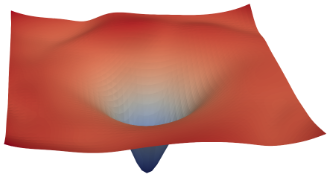
\includegraphics[width=8cm]{./images/loss-short}
\caption{}
\label{fig:resloss2}
\end{subfigure}
\caption{Na slici \protect\subref{fig:resloss1} je prikazana funkcija cilja bez korištenja preskočnih veza dok je na slici \protect\subref{fig:resloss2} prikazana funkcija cilja nakon ubacivanja preskočnih veza u model. Prikazi su preuzeti iz \cite{NIPS2018_7875}.}
\end{figure}
\subsection{MobileNets}
MobileNets predstavljaju razred efikasnih modela za mobilne i ugradbene sustave namijenjene za računalni vid. Baziraju se na arhitekturi koja koristi dubinski separabilne konvolucije za izgradnju efiksanih dubokih modela \cite{mobilenets}. \par Arhitektura se ističe po tome što obične konvolucijske slojeve mijenja sa dva konvolucijska sloja pri čemu prvi sloj ima ulogu nezavisnog filtriranja pojedinih mapa značajki, a drugi ulogu kombiniranja značajki imeđu različitih kanala ulaza.  Kombinaciju takva dva konvolucijska sloja nazivamo dubinski separabilna konvolucija. Prvi konvolucijski sloj je grupni konvolucijski sloj sa grupom veličine 1, a drugi točkasti konvolucijski sloj \engl{pointwise convolutional layer}. U MobileNet arhitekturi, grupni konvolucijski sloj primjenjuje zasebnu jezgru za svaki ulazni kanal. Točkasti konvolucijski sloj koristi jezgru \verb|1x1| kojim kombinira izlaze grupnog konvolucijskog sloja. 
\begin{figure}[htp]

\centering
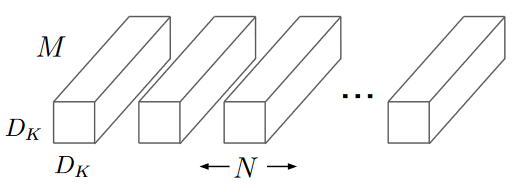
\includegraphics[width=.3\textwidth]{./images/mn1}\hfill
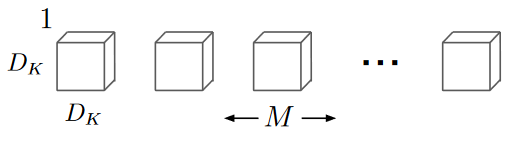
\includegraphics[width=.3\textwidth]{./images/mn2}\hfill
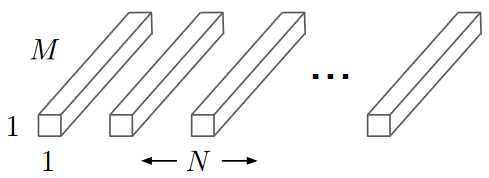
\includegraphics[width=.3\textwidth]{./images/mn3}

\caption{Standardna konvolucija (lijevo) je zamijenjena grupnom konvolucijom (sredina) i točkastom konvolucijom (desno). Slika je preuzeta iz \cite{mobilenets}.}
\label{fig:mobnet}
\end{figure}
\par
Standardna konvolucija ima sljedeću složenost:
\begin{equation}
D_K * D_K * M * N * D_F * D_F
\end{equation}
gdje je $N$ broj ulaznih kanala, $M$ broj izlaznih kanala, $D_k$ \verb|x| $D_k$ dimenzija jezgre (uz pretpostavku da koristimo kvadratnu jezgru) i $D_f$ \verb|x| $D_f$ prostorne dimenzije izlazne mape značajki. Kod grupnog konvolucijskog sloja imamo zasebnu jezgru za svaki ulazni kanal. Tada je njegova složenost: 
\begin{equation}
D_K * D_K * M *  D_F * D_F
\end{equation} Dubinski konvolucijski sloj je efikasan ali radi samo filtraciju ulaznih kanala, ne i njihovu kombinaciju. Točkasti konvolucijski sloj radi linearnu kombinaciju izlaza dubinskog konvolucijskog sloja sa \verb|1 x 1| konvolucijom. Ukupna složenost dubinski separabilne konvolucije je:
\begin{equation}
D_K * D_K * M *  D_F * D_F + M * N * D_F * D_F
\end{equation}
\par
U MobileNet arhitekturi svi su konvolucijski slojevi dubinski separabilni osim prvog konvolucijskog sloja. Prvi konvolucijski sloj prati 13 blokova dubinski separabilnih slojeva. Iza svakog konvolucijskog sloja dolazi sloj normalizacije po grupi i aktivacijska funkcija zglobnica.
\par
MobileNet uvodi dva hiperparametra kojima se omogućuje da model bude još manji i brži iako time gubi na točnosti što ovisno o problemu koji rješavamo može biti prihvatljivo. Prvi hiperparametar je multiplikator dubine $\alpha \in (0,1]$ koji smanjuje broj ulaznih kanala u konvolucijski  sloj, odnosno dubinski separabilna konvolucija tada ima sljedeću složenost:
\begin{equation}
D_K * D_K * \alpha M *  D_F * D_F + \alpha M * \alpha N * D_F * D_F
\end{equation} 
Ovaj parametar smanjuje složenost sloja i smanjuje broj parametara za faktor oko $\alpha^2$. Drugi hiperparametar je multiplikator rezolucije $\rho \in (0,1]$ koji smanjuje prostorne dimenzije mapi značajki. Dubinski separabilna konvolucija tada ima složenost:
\begin{equation}
D_K * D_K *  M *  \rho D_F * \rho D_F +  M *  N * \rho D_F * \rho D_F
\end{equation}  
\par
MobileNet ima nekoliko novijih verzija koja nose određena poboljšanja u odnosu na originalnu arhitekturu. Tako se MobileNetV2 arhitektura bazira na invertiranoj rezidualnoj strukturi. 
\par
Arhitektura koristi Relu6 aktivacijsku funkciju koja je slična zglobnici. Računa se pomoću formule $y = min(max(0,x),6)$. Koristi se zbog robusnosti kod izračuna sa malom preciznosti.
\begin{figure}[htb]
\centering
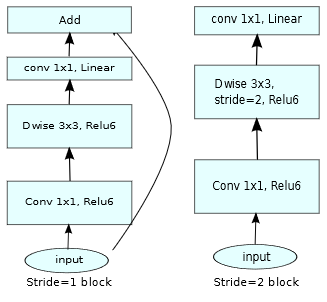
\includegraphics[width=8cm]{./images/mnv2}
\caption{Prikaz invertiranog rezidualnog bloka sličnog rezidualnim blokovima koji su uvedeni u MobileNetV2 arhitekturu kao značajno poboljšanje u odnosu na MobileNet arhitekturu. Slika lijevo označava niz slojeva koji se koristi kad je pomak jednak 1 ili je dubina izlaznog sloja jednaka dubini ulaznog sloja. U tom slučaju se koristi preskočna veza. Slika desno označava slučaj kad je pomak jednak 2 ili je dubina izlazne mape značajki različita od dubine ulazne mape značajki. Tada se ne koristi preskočna veza.  Primjetimo invertirani bottleneck dizajn, gdje se redom koriste konvolucije 1x1, 3x3 i 1x1. Prikaz je preuzet iz \cite{mobilenetv2}.}
\label{fig:mobnetv2}
\end{figure}\par
Na slici \ref{fig:mobnetv2} je prikazana osnovna gradivna jedinica MobileNetV2 arhitekture. Prvi konvolucijski sloj \verb|1x1| se koristi za ekspanziju dimenzija, a zadnji konvolucijski sloj \verb|1x1| se koristi za ponovno sažimanje dimenzija. Primjetimo da je ovo obrnuto od bottleneck arhitekture koja se koristi u rezidualnoj arhitekturi. Za prve dvije konvolucije se koristi aktivacija ReLU6 dok se za zadnju konvoluciju koristi linearna aktivacijska funkcija. Korištenje linearne aktivacije je ključno kako bi sprječili nelinearnosti da unište previše informacija, što se primjerice može dogoditi kod aktivacijske funkcije zglobnice.

\section{Modeli sa sažimajućim značajkama}
Prva arhitektura za klasifikaciju videa koju ćemo implementirati u sklopu našeg rada je arhitektura sažimajućih značajki \engl{feature pooling architecture}. Iz svakog okvira videa se uz pomoć bloka konvolucijskih slojeva ekstrahiraju značajke. Potom se raznim kombinacijama slojeva sažimanja kombiniraju izlazi ekstraktora značajki za svaki pojedini okvir. Rad \cite{feature-pooling} predlaže nekoliko različitih načina kako kombinirati značajke. Na slojeve potrebne za kombinaciju značajki se dodaje klasifikator koji daje konačan izlaz modela. 
\begin{figure}[htb]
\centering
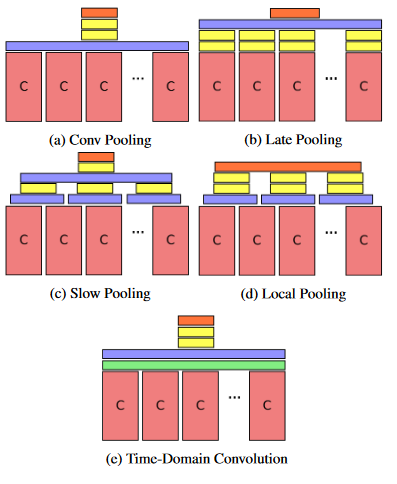
\includegraphics[width=8cm]{./images/feature-pooling}
\caption{Prikaz različitih feature-pooling arhitektura. Crvena, plava, žuta, narančasta i zelena boja redom označavaju konvolucijske slojeve, sloj sažimanja, potpuno povezani sloj, softmax sloj, vremensku konvoluciju. Prikaz je preuzet iz \cite{feature-pooling}.}
\label{fig:rfeature-pooling}
\end{figure}
Conv Pooling arhitektura na izlaz bloka konvolucijskih slojeva postavlja sloj sažimanja maksimumom po vremenskoj domeni. Late Pooling na blok konvolucijskih slojeva dodaje dva potpuno povezana sloja. Nakon drugog potpuno povezanog sloja se dodaje sloj sažimanja po vremenskoj domeni te se računa izlaz modela. Slow pooling prvo kombinira značajke manjeg vremenskog prozora, na koji se dodaje potpuno povezani sloj te sloj sažimanja po vremenskoj domeni. Na taj sloj se dodaje još jedan potpuno povezan sloj i konačno se računa izlaz modela. Local Pooling je sličan prethodnoj arhitekturi. Razlika je u tome što ima samo jedan sloj sažimanja na koji se dodaju dva potpuno povezana sloja te se računa izlaz modela. Time-Domain Convolution koristi vremensku konvoluciju za kombinaciju značajki pojedinih okvira. Na taj sloj se dodaje sloj sažimanja i dva potpuno povezana sloja nakon kojih se računa izlaz modela. 
\par
U arhitekturama se kao sloj sažimanja koristi sloj sažimanja maksimumom. To nije nužno samo po sebi, ali se pokazalo da sloj sažimanja prosjekom i potpuno povezani sloj kao sloj sažimanja imaju problema sa učenjem zbog velikog broja gradijenata koje generiraju. U sklopu ovog rada smo odlučili isprobati Conv Pooling arhitekturu jer se pokazalo da od svih gore navedenih arhitektura postiže najbolje rezultate \cite{feature-pooling}.
\newpage
\section{SlowFast arhitektura}
\label{section:slowfast-cite}
Druga arhitektura koju razmatramo i implementiramo u sklopu našeg rada je Brzo-Spora \engl{SlowFast} arhitektura. Glavna pretpostavka na kojoj se bazira ova arhitektura je da su u videu sporiji pokreti izgledniji od brzih pokreta, što je i istina ako uzmemo u obzir da je većina svijeta oko nas koju percipiramo statična. Ako razmatramo brid nekog objekta koji se pomiče u proizvoljnom smjeru, možemo percipirati samo kretanje koje je okomito na taj brid, iako je moguće da postoji komponenta kretanja u tangencijalnom smjeru s obzirom na promatrani brid. To se događa zato jer pokret percipiramo pomoću promjene intenziteta piksela koja se u tangencijalnom smjeru nije promijenila. Problem nazivamo problemom otvora kamere.
\begin{figure}[htp]
\begin{subfigure}{.5\textwidth}
\centering
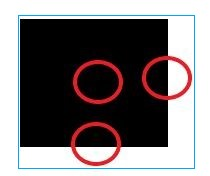
\includegraphics[width=.5\textwidth]{./images/mov1-p}\hfill
\caption{Prikaz scene prije pomicanja objekta.}
\label{fig:mov-1}
\end{subfigure}
\begin{subfigure}{.5\textwidth}
\centering
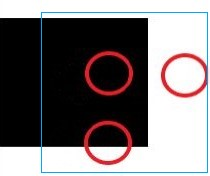
\includegraphics[width=.5\textwidth]{./images/mov2-p}\hfill
\caption{Prikaz scene nakon pomicanja objekta u desno.}
\label{fig:mov-2}
\end{subfigure}
\caption{Crni objekt sa slike \protect\subref{fig:mov-2} se pomaknuo u lijevo u odnosu na sliku \protect\subref{fig:mov-a}. Taj pomak je moguće percipirati u području desnog kruga, ali ne i u području lijevog i donjeg kruga. Taj problem nazivamo problemom otvora kamere.}
\label{fig:apeture}
\end{figure}
Kako naše oko prostorne i vremenske značajke različito percipira, rad pretpostavlja da bi model za klasifikaciju videa mogao jednako tako različito tretirati prostorne i vremenske značajke videa. Konkretno, ako razmatramo problem klasifikacije videa, kategorička prostorna semantika prikazanog sadržaja se sporo mijenja. Odnosno, na videu gdje je prikazano mahanje ruke, ruka ostaje ruka tijekom cijelog videa - objekt se sporo mijenja, dok se sama radnja mahanja ruke odvija relativno brzo. Za raspoznavanje ruke kao objekta nam je potrebno puno manje okvira videa nego za raspoznavanje mahanja ruke kao pokreta. Upravo tu činjenicu želimo iskoristiti u našoj arhitekturi. Ljudsko oko ima dvije vrste stanica, od kojih je $~80\%$ Parvocellularnih stanica (P-stanice) i $~15-20\%$ Magnocellularnih stanica (M-stanice). M-stanice su zadužene za brze vremenske promjene i nisu osjetljive na boju i prostorne detalje, dok su P-stanice zadužene za prostorne detalje i slabo reagiraju na brze promjene. Analogno tim spoznajama, u sklopu modela imamo dvije staze, jednu koja će obrađivati okvire uzrokovane visokom frekvencijom i drugu koja će obrađivati okvire uzorkovane nižom frekvencijom \cite{slow-fast}. Prvu stazu nazivamo "Brza" staza, dok drugu nazivamo "Spora" staza.
\par
"Spora" staza služi za hvatanje semantičke informacije iz videa, za koju je dovoljan jedan ili nekoliko okvira iz videa. "Brza" staza služi za hvatanje brzog pokreta u videu, promjene koje se odvijaju između gotovo svakog okvira. Ta staza koristi okvire koji su uzorkovani frekvencijom koja je $\alpha$ puta veća od frekvencije korištene za "Sporu" stazu. "Brza" staza je dizajnirana tako da ima $\beta$ puta manje kanala (dubina mape značajki) od "Spore" staze kako bi imala slabiju mogućnost percipiranja prostornih informacija što je zadatak "Spore" staze. Staza je namjerno tako dizajnirana kako bi ubrzali izračun, na izračune u "Brzoj" stazi otpada 20\%  ukupnog izračuna modela. Na slici \ref{fig:slowfastdiag} vidimo prikaz kako izgleda SlowFast arhitektura.
\begin{figure}[htp]

\centering
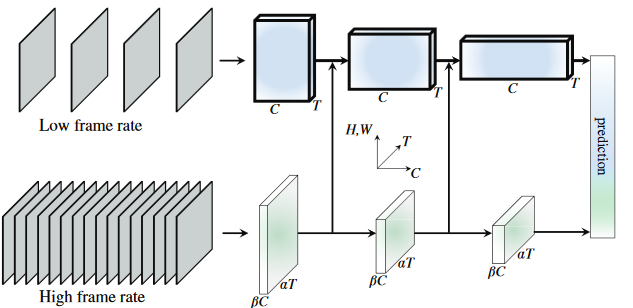
\includegraphics[width=\textwidth]{./images/slow-fast-diag}\hfill

\caption{Prikaz SlowFast arhitekture. Gornja stazu nazivamo Spora staza, a donju Brza staza prema frekvenciji uzorkovanja okvira. Informacije iz Brze staze ugrađujemo u Sporu stazu pomoću lateralnih veza u različitim dijelovima arhitekture. Tenzori se transformiraju sa 3D konvolucijskim slojevima. Iako je arhitektura namijenjena za obradu okvira iz videa, na ulaz pojedinih staza je moguće postaviti značajke iz nekog drugog modela.  Prikaz je preuzet iz \cite{slow-fast}.}
\label{fig:slowfastdiag}
\end{figure}
\par
Kako bi dali modelu priliku da ugradi informacije iz jedne staze u drugu, koristimo lateralne veze. Orginalni rad predlaže nekoliko različitih načina kako obaviti ugradnju informacija. U okviru naših eksperimenata ćemo isprobati sljedeći način. Koristit ćemo jednosmjernu vezu koja ugrađuje informacije iz "Brze" staze u "Sporu" stazu. Pokazuje se da dvosmjerna veza radi jednako dobro kao i jednosmjerna veza pa smo izabrali jednostavniju opciju. Ako je dimenzija mape značajki "Spore" staze ${T, S^2,C}$, tada je dimnezija "Brze" staze ${\alpha T, S^2, \beta C}$, gdje je $T$ broj okvira, $S$ prostorna dimenzija i $C$ broj kanala mape značajki. Za ugradnju koristimo vremensku konvoluciju sa $2\beta C$ jezgri dimenzija \verb|{5,1^2}|, pri čemu je veličina jezgre iskazana kao \verb|{T,S^2}| gdje je $T$ veličina jezgre po vremenskoj osi, \verb|S^2| veličine jezgre po prostornim osima. Za operaciju konvolucije se koristi pomak $\alpha$. U našim eksperimentima koristimo ResNet18 prilagođen za trodimenzionalne podatke. Nakon svakog rezidualnog bloka dodajemo lateralnu vezu koja ugrađuje informacije iz "Brze" staze u "Sporu" stazu. Iza zadnjeg rezidualnog bloka umjesto lateralne veze na svaku stazu dodajemo sloj globalnog sažimanja prosjekom. Dobivena dva vektora iz svake staze konkateniramo i dovodimo na ulaz potpuno povezanog sloja sa brojem neurona jednakom broju semantičkih razreda skupa podataka sa "softmax" aktivacijskom funkcijom kojeg koristimo za klasifikaciju.
\chapter{Programska izvedba}
\section{Keras}
Keras je programski okvir visoke razine za strojno učenje. Odlikuje ga jednostavnost uporabe, modularnost i proširivost. Radi na brojnim platformama poput Tensorflowa, Theana i PlaidMLa. Omogućuje brzo i jednostavno eksperimentiranje sa dubokim modelima. Uz PyTorch je jedan od popularnijih okvira za strojno učenje. Tensorflow 2.0 je usko vezan uz Keras i velika većina Tensorflow modela je pisana upravo u Kerasu. Keras iznosi dva programska sučelja za kreiranje modela.
\par
Programsko sučelje \verb|tf.keras.Sequential| grupira niz slojeva u instancu razreda \verb|tf.keras.Model|. Pogodno je za implementaciju modela koji imaju jedan ulaz i jedan izlaz. U sljedećem isječku vidimo model koji se sastoji od dva potpuno povezana sloja i koji je izgrađen ovim sučeljem.
\lstinputlisting[language=Python]{./examples/sequential.py}
Model se izrađuje dodavanjem slojeva modelu pomoću \verb|model.add| funkcije. Prilikom kreiranja prvog sloja u modelu, potrebno je predati i \verb|input_shape| argument. Pri dodavanju ostalih slojeva nije potrebno predavati dimenzije podataka već ih Keras sam računa. 

Funkcijsko programsko sučelje je fleksibilnije od \verb|tf.keras.Sequential| sučelja. Za razliku od navedenog sučelja, dopušta kreiranje modela sa više ulaza i izlaza. Potrebno je definirati ulazni sloj za svaki ulaz sa potrebnim dimenzijama. U sljedećem isječku koda vidimo model koji je izgrađen sa dfunkcijskim sučeljem.
\lstinputlisting[language=Python]{./examples/functional.py}
\par
\par
Svaki Keras model ima metodu \verb|summary()| koja prikazuje veličinu mape značajki nakon svakog sloja i broj parametara, a u modelima izgrađenim sa funkcijskim programskim sučeljem i slojeve s kojim je neki sloj povezan, što su informacije koje su veoma korisne prilikom procesa pronalaženja grešaka u kodu.
\section{Keras generator podataka}
\label{section:data-gen}
Prilikom implementacije naših modela, mnogo problema smo imali sa pripremom podataka za treniranje pomoću Kerasa. Keras nudi mnogobrojne generatore podataka koji omogućavaju jednostavno učitavanje skupova podataka koji sadrže slike, ali ne nudi generatore koji učitavaju video podatke. Zbog toga smo morali sami pristupiti implementaciji takvog generatora. Podatke smo pokušali učitati u model na dva načina. 
\par
Prvi način koji smo isprobali je uzorkovati potreban broj okvira iz videa prije samog treniranja. Ovaj je pristup dobar jer ubrzava učenje - nije potrebno trošiti vrijeme na uzorkovanje okvira tijekom treniranja, te omogućava pohranjivanje ekstrahiranih značajki iz video okvira pomoću kralježničkog modela treniranog na drugom problemu. Mana ovog pristupa je što generira veliki broj datoteka na disku, što nam je uz činjenicu da smo na Google Disku imali ograničen prostor za pohranu, predstavljalo velik problem.
\par
Drugi način koji smo isprobali je uzorkovati okvire iz videa tijekom samog treniranja. Prije samog treniranja smo učitali liste sa putanjama do video podataka i napravili smo train/valid/test podjele na temelju tih podataka. Prilikom dohvata podatka tijekom treniranja, učitali smo traženi video i iz njega pomoću \verb|cv2| paketa uzorkovali željeni broj okvira iz videa. Augmentaciju podataka smo obavljali tako da smo na svaki niz okvira primjenili slučajnu transformaciju. Iako je ovaj način dohvata podataka sporiji od prvog načina, pokazalo se da je za naše eksperimente bolji. 
\newpage
\section{Modeli sa sažimajućim značajkama}
Razvili smo arhitekturu sa sažimajućim značajkama pomoću tf.keras.Sequential sučelja. Kako bismo primjenili isti kralježnički model za ekstrahiranje iskoristili smo tf.keras.layers.TimeDistributed sloj. Taj sloj će primjeniti sloj koji omeđuje na svaki vremenski okvir. Ako želimo iskoristiti potpuno povezani sloj sa 10 neurona na svaki okvir iz videa, pomoću \verb|tf.keras.layers.TimeDistributed| sloja ćemo to napraviti na sljedeći način: \verb|TimeDistributed(Dense(10))|. Bitno je primjetiti da su težine između potpuno povezanih slojeva dijeljene, odnosno da se na svaki okvir videa primjenjuje isti potpuno povezani sloj. U okviru rada smo implementirali Conv Pooling arhitekturu iz rada \cite{feature-pooling}, gdje se operacija sažimanja provodi nakon zadnjeg konvolucijskog sloja kroz okvire videa. U sljedećem isječku je prikazana implementacija te arhitekture.
\lstinputlisting[language=Python]{./examples/feature_pooling.py}
Iz kralježničkog modela smo uzeli sve slojeve do zadnjeg konvolucijskog sloja uključivo, pri čemu je model prethodno treniran na Imagenet skupu podataka. Tijekom treniranja naših modela, dopustili smo pretreniranim težinama iz kralježničkih modela da se dodatno prilagode problemu koji rješavamo. Izvodili smo eksperimente i tako da smo fiksirali predtrenirane težine, ali smo na taj način ostvarivali nešto lošiji rezultat.
\newpage
\section{SlowFast model}
Ovu arhitekturu smo implementirali pomoću Kerasovog funkcijskog sučelja. Prvi sloj u modelu je sloj kojim uzorkujemo okvire koji su dovedeni na ulaz kako bismo dobili "Sporu" stazu. U sljedećem isječku koda vidimo funkciju koju koristimo za uzorkovanje okvira. Funkcija \verb|prepare_input| vraća Kerasov lambda sloj koji obavlja željenu operaciju. Kao argument prima faktor $\alpha$ koji je objašnjen u poglavlju \ref{section:slowfast-cite}.
\lstinputlisting[language=Python]{./examples/slow-fast-slow.py}
Nakon ovog sloja, efektivno imamo dvije staze za obradu podataka. Staze obrađujemo zasebnim slojevima uz iznimku slojeva koje koristimo za spajanje podataka iz jedne staze u drugu. U našim eksperimentima spajamo informacije iz brze staze u sporu. Spajanje provodimo uz pomoć konvolucijskog sloja koji radi sa 3D podacima koji na ulaz prima mapu značajki Brze staze. Taj sloj ima $2 \beta C$ jezgri, svaka jezgra je dimenzija \verb|5x1x1| uz pomak $\alpha$ kao što je objašnjeno u poglavlju \cite{section:slowfast-cite}. Izlaz iz tog konvolucijskog sloja konkateniramo na mapu značajki Spore staze. Primjerice, ako je mapa značajki Spore staze dimenzija \verb|4x56x56x256|, tada je dimenzija mape značajki Brze staze \verb|32x56x56x32|. Izlaz konvolucijskog sloja koji koristimo za spajanje je dimenzija \verb|4x56x56x64|, te je izlaz samog sloja za spajanje nakon konkatenacije  \verb|4x56x56x320|.
\par
Pošto koristimo ResNet18 kao kralježničku arhitekturu, navedeno spajanje obavljamo nakon svakog ResNet gradivnog bloka. Izuzetak je zadnji ResNet gradivni blok, kad spajanje obavljamo nešto drugačije. Mapu značajki sa svake staze dovodimo na globalni sloj sažimanja prosjekom, što vidimo na sljedećem isječku koda. 
\lstinputlisting[language=Python]{./examples/slow-fast-final.py}
Mapa značajki dobivena nakon zadnjeg rezidualnog bloka za "Sporu" stazu je u liniji 1 prethodnog isječka dovedena na ulaz od sloja globalnog sažimanja prosjekom, dok je u liniji 2 mapa značajki dovedena na ulaz sloja globalnog sažimanja prosjekom za "Brzu" stazu.  
Izlaze tih slojeva potom konkateniramo na liniji 4, obavljamo dropout na liniji 5 i dovodimo na potpuno povezani sloj sa brojem neurona jednakom broju razreda skupa podataka na liniji 6. Koristimo softmaks aktivacijsku funkciju kao aktivacijsku funkciju zadnjeg potpuno povezanog sloja. Izlaz modela shvaćamo kao vjerojatnost pripadnosti ulaznog podatka pojedinom razredu.
\par
Nakon svakog konvolucijskog sloja koje koristimo u ovoj arhitekturi, dolazi sloj normalizacije po grupama. Za aktivacije konvolucijskih slojeva koristimo aktivacijsku funkciju zglobnicu. 
\chapter{Skupovi podataka za učenje}
Danas postoji mnogo standardnih skupova podataka za koji se koriste za evaluaciju modela za klasifikaciju videa. U najpoznatije skupove ubrajamo UCF-101, Kinetics-400, Kinetics-600, Charades, YouTube-8M. Neki od skupova su doista impresivni, YouTube-8M skup sadrži preko 8 milijuna videa ukupnog trajanja preko 500 000 sati, pri čemu je svaki video iz skupa označen s jednim od 4803 razreda.
\section{UCF-101}
Skup sadrži kratke video isječke koji predstavljaju razne ljudske aktivnosti \cite{ucf101}. Isječci su označeni sa ukupno 101 razredom pri čemu je svaki isječak označen samo jednim razredom. Aktivnosti koje pronalazimo u ovom skupu su doista raznovrsne, od raznih sportova poput raftinga, do radnji kao što su šišanje kose i nanošenje šminke. Skup ukupno sadrži 13 320 snimaka ukupnog trajanja preko 27 sati, pri čemu se 9537 videa nalazi u skupu za treniranje te 3783 videa u testnom skupu. 
\par
Glavne prednosti koje ovaj skup ima nad prethodnim skupovima poput skupova UCF-50 i HMDB51 su povećanje broja semantičkih razreda u skupu i povećanje varijacije među razredima korištenjem raznovrsnijih ljudskih aktivnosti \cite{ucf101}. Najveća mana skupa je što je iz jednog videa gdje se primjerice pokazuje osoba koja četka kosu, izvađeno i do 7 video isječaka. Skup je organiziran tako da su isječci unutar jednog razreda podijeljeni u 25 grupa. Unutar svake grupe se nalazi 4-7 isječaka koji imaju slične značajke poput pozadine i subjekta koji vrše aktivnost. Zbog činjenice da je većina aktivnosti unutar jedne grupe snimano istom kamerom sa sličnim ambijentalnim uvjetima, imamo relativno malenu varijaciju među podacima jednog razreda \cite{kinetics}.
\par
Danas se pojavljuje sve manje modela koji prikazuju rezultate na ovom skupu jer postoje noviji skupovi koji nemaju probleme skupa UCF-101\footnote{Između ostalih, Kinetics-400 smatramo standardnim skupom za evaluaciju modela za klasifikaciju videa}, ali zbog računalnih ograničenja će ovaj skup dobro poslužiti za ispitivanje naših modela.
\begin{figure}[htp]

\centering
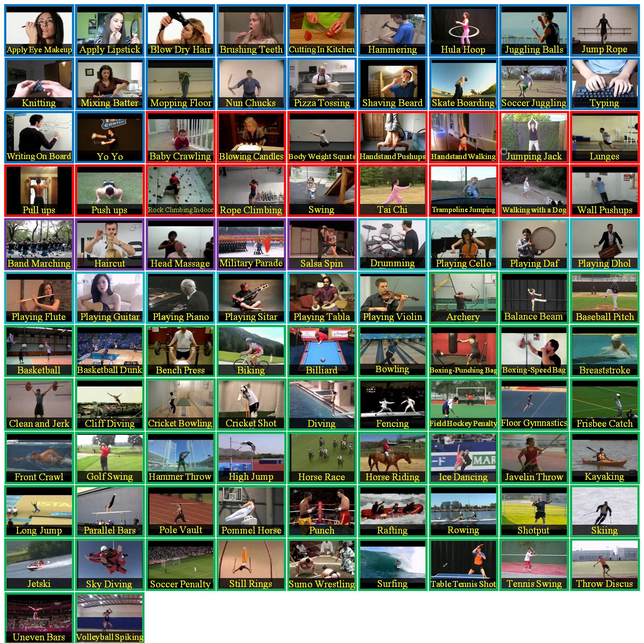
\includegraphics[width=\textwidth]{./images/ucf-101}\hfill

\caption{Prikaz svih razreda skupa UCF-101. Prikaz je preuzet iz \cite{ucf101}.}
\label{fig:ucf101}
\end{figure}
\chapter{Eksperimenti}
U okviru ovog poglavlja opisujemo eksperimente koje smo provodili u sklopu ovog rada, te koje smo rezultate ostvarili. Provodili smo klasifikaciju videa iz UCF-101 skupa podataka pomoću dvije različite arhitekture: arhitektura sa sažimajućim značajkama i SlowFast arhitektura.
\section{Metrike}
Metrike predstavljaju objektivne mjere za evaluaciju performansi naših modela. Najpopularnija metrika koja se koristi za evaluaciju modela za klasifikaciju je točnost klasifikacije. Točnost klasifikacije računamo na sljedeći način:
\begin{equation}
\text{Točnost} = \frac{\text{Broj točnih predviđanja modela}}{\text{Ukupan broj primjera}}
\end{equation}
Kako bismo mogli koristiti točnost kao metriku, naš skup podataka mora biti balansiran, odnosno moramo imati podjednak broj primjera unutar svakog razreda. Skup koji koristimo u našim eksperimentima je dobro balansiran.
\par
Osim točnosti klasifikacije, u literaturi često susrećemo i \verb|top-k| točnost. \verb|Top-k| točnost se razlikuje od obične točnosti po tome što se točnim predviđanjem smatra slučaj kad je točan razred unutar \verb|k| najvećih vjerojatnosti izlaza modela.
\par
Rezultate koje smo postigli u sklopu naših eksperimenata evaluiramo pomoću metrika top-1 točnosti i top-3 točnosti.
\section{Povećanje skupa za učenje}
Kako radimo sa relativno malim skupom podataka, u našim eksperimentima smo odlučili koristiti povećanje skupa za učenje \engl{data augmentation} kako bismo poboljšali rezultate klasifikacije i smanjili mogućnost pretreniranja modela. Za povećanje skupa smo koristili instancu Kerasovog ImageDataGeneratora, koju smo kreirali sa željenim transformacijama. U sljedećem isječku je prikazan proces kreiranja instance ImageDataGeneratora koji koristimo za povećanje skupa za učenje.
\lstinputlisting[language=Python]{./examples/augmentation.py}
Stvoreni objekt smo predali generatoru podataka. Na kraju svake epohe smo pomoću objekta kreirali nasumičnu transformaciju za svaki video što je vidljivo na sljedećem isječku.
\lstinputlisting[language=Python]{./examples/augmentation2.py}
Tijekom treniranja, iz svakog videa smo uzorkovali željeni broj okvira, te smo na svaki okvir iz videa primjenili istu pripremljenu transformaciju. 
\lstinputlisting[language=Python]{./examples/augmentation3.py}
\section{Rezultati}
U ovom poglavlju prikazujemo rezultate naših eksperimenata. Svi eksperimenti su provedeni na Google Colab platformi. Google Colab kod izvodi na virtualnom stroju na kojem nam je dostupno 12 GB radne memorije. Za treniranje nam je dostupna i grafička kartica. Ovisno o tome koji je virtualni stroj dostupan, na raspolaganje možemo dobiti Tesla K80 grafičku karticu i Tesla P100 grafičku karticu. Kako bi mogli trenirati modele neovisno o grafičkoj kartici koju dobijemo na raspolaganje sa istom veličinom mini grupe, koristimo veličinu mini grupe 8 za sve eksperimente.
\subsection{Modeli sa sažimajućim značajkama}
Eksperimentirali smo sa različitim kralježničkim arhitekturama kako bismo pokušali dobiti što bolji rezultat. Originalni rad \cite{feature-pooling} koristi nešto starije arhitekture, AlexNet i GoogleNet. Izabrali smo novije arhitekture, ResNet18, MobileNet i MobileNetV2 kako bi povećali šansu uspjeha.
\par
Koristili smo modele koji su predtrenirani na Imagenet skupu podataka kako bi ubrzali treniranje. Koristili smo Adam optimizacijski postupak sa stopom učenja $10^{-3}$. Model smo trenirali 20 epoha, pri čemu smo koristili rano zaustavljanje kako pohranili model koji najbolje generalizira.
\par
UCF-101 definira tri podjele skupa na skup za treniranje i testiranje koje se koriste za prijavu rezultata. Podjele su napravljene tako da su svi podaci iz skupa nasumično podijeljeni u skup za treniranje i skup za testiranje pri čemu 70\% podataka iz skupa ide u skup za treniranje. Postupak je ponovljen tri puta.  Rezultati se obično prijavljuju kao prosjek točnosti na testnom skupu iz svake od navedenih podjela. Zbog ograničenog vremena dostupnog za treniranje na Google Colabovim grafičkim karticama, rezultate prijavljujemo na samo prvoj od navedene tri podjele. Svi eksperimenti u ovom radu su provedeni sa 32 okvira uzorkovanih iz videa. Okvire smo uzorkovali drugom metodom koja je opisana u \ref{section:data-gen}. Uzorkovali smo pomoću cv2 paketa na način da smo koristili korak uzorkovanja koji je izračunat kao ukupni $\text{broj okvira u videu} / \text{željeni broj okvira}$. U literaturi \cite{feature-pooling} su provedeni eksperimenti i gdje je uzorkovano samo prvih 30 okvira videa. Tablica \ref{tbl:results} prikazuje postignute rezultate. Prvi stupac tablice označava koja je kralježnička arhitektura u modelima sažimajućih značajki korištena. Drugi stupac prikazuje ostvarenu \verb|top-1| točnost, a treći stupac ostvarenu \verb|top-3| točnost. U tablici je vidljivo da najbolju \verb|top-1| točnost ostvaruje model koji koristi MobileNetV2 kao kralježničku arhitekturu.
\begin{table}[htb]
\caption{Prikaz ostvarene top-1 i top-3 točnosti na testnom skupu UCF-101 skupa korištenjem različitih kralježničkih arhitektura u Conv Pooling arhitekturi sažimajućih značajki.}
\label{tbl:results}
\centering
\begin{tabular}{llr} \\ \toprule
backbone & top-1 točnost & top-3 točnost \\ \midrule
$\text{ResNet18}$ & 66.65\% & 81.60\% \\
$\text{MobileNet}$ & 70.54\% & 86.63\% \\
$\text{MobileNetV2}$ & 71.73\% & 83.75\% \\ \bottomrule
\end{tabular}
\end{table}
\par
Proveli smo i eksperiment sa 10 okvira uzorkovanih iz videa na MobileNetV2 arhitekturi i postigli smo top-1 točnost od $68.76\%$ i top-3 točnost od $80.85\%$, što je slabiji rezultat od modela koji na ulazu prima 32 okvira. Ovaj rezultat je očekivan jer model koji na ulazu prima 32 okvira vidi više konteksta iz jednog videa što je prednost za klasifikaciju.
\par
Rezultati ostvareni modelima sa sažimajućim značajkama su blizu rezultata koji su postignuti u originalnom radu. U originalnom radu je na istom skupu sa Conv Pooling arhitekturom postignut rezultat od 80.8\% uz prijavljenu \verb|top-1| točnost na test skupu koja je dobivena trostrukom unakrsnom validacijom. Mi najbolji rezultat ostvaruje modelom koji koristi MobileNetV2 kao backbone, što smo i očekivali s obzirom na to da je arhitektura već nadmašila rezultat MobileNet arhitekture na problemu klasifikacije slika \cite{mobilenetv2}. Pretpostavljamo da bi daljnjim podešavanjem hiperparametara uspjeli ostvariti bolji rezultat. Pri evaluaciji bi trebalo koristiti sve tri predložene podjele kao što je napravljeno u radu, ako je to moguće. U originalnom radu je prijavljena točnost od $80.8\%$ sa kralježničkim arhitekturama sa većim brojem parametara. Također, prijavljen je rezultat od $87.6\%$ uz korištenje optičkog toka. U sklopu budućih eksperimenata bi svakako bilo zanimljivo ispitati i kako bi se naši modeli ponašali uz korištenje optičkog toka. U tom slučaju bi očekivali poboljšanje rezultata. Modele naučene sa optičkim tokom bi bilo zanimljivo usporediti sa tehnikama koje su predložene u radu \cite{saric20cvpr} koje nadmašuju rezultate modela sa optičkim tokom na problemu semantičke segmentacije okvira u budućnosti. Kako bi mogli trenirati modele sa većim mini-grupama u budućim eksperimentima bi bilo zanimljivo isprobati tehniku pohranjivanja gradijenata koja bi omogućila našim modelima niže memorijsko zauzeće. Takve bi modele mogli trenirati sa većim veličinama mini grupe što bi vjerojatno dovelo i do stabilnijeg učenja.
\subsection{SlowFast model}
Testirali smo performanse SlowFast modela na testnom skupu UCF-101 skupa. Implementirali smo ResNet18 verziju prilagođenu radu s 3D podacima. Za razliku od prethodnog modela, ovaj model nismo predtrenirali na Imagenet skupu podataka kao što je i predloženo u originalnom radu \cite{slow-fast}.  Koristili smo Adam optimizacijski postupak sa stopom učenja $10^{-4}$. Model smo trenirali 40 epoha, pri čemu smo kao i kod prethodnog modela koristili rano zaustavljanje kako bi pohranili model koji najbolje generalizira. Ostvarili smo od $42.95\%$ \verb|top-1| točnost i $61.77\%$ \verb|top-3| točnost na testnom skupu.
\par
SlowFast arhitektura je ostvarila lošiji rezultat što nismo očekivali, te pretpostavljamo da je moguće da je rezultat nastao uslijed lošeg izbora hiperparametara ili zbog previđene greške u implementaciji. Trebali bi nastaviti eksperimentirati sa hiperparametrima kako bi poboljšali rezultat.

\subsection{Slike rezultata}
U nastavku dajemo nekoliko uzoraka iz testnog skupa sa pripadajućim predikcijama modela s kojim smo ostvarili najbolji rezultat, MobileNetV2.
\par
Za video podatke prikazane slikama \ref{fig:playingpiano} i \ref{fig:rockclimbing} vidimo da model sa velikom sigurnošću tvrdi da je na videim prikazana radnja sviranja klavira i radnja penjanja po umjetnoj stijeni. Radnje su specifične i nisu slične ostalim radnjama u skupu pa model nema većih problema sa prepoznavanjem točnih radnji. Za video prikazan slikom \ref{fig:mixing} vidimo da model točno predviđa da je na videu prikazana radnja mješanja hrane ali sa manjom sigurnošću. Razlog tomu je da model ima problema sa razlikovanjem radnji koje se događaju pod sličnim uvjetima. Za video prikazan slikom \ref{fig:hammering} model točno tvrdi da je na videu prikazano udaranje čekićem. Ovaj rezultat je zanimljiv jer čekić nije lako uočiti i jer video sadrži dvije osobe što nije specifično za samu radnju.
\begin{figure}[htp]
\begin{subfigure}{\textwidth}

\centering
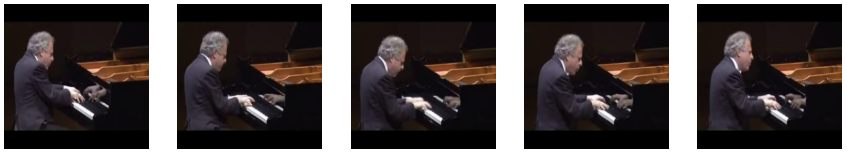
\includegraphics[width=\textwidth]{./images/playing_piano}\hfill

\caption{Model je predvidio točan razred "Playing Piano", izlaz modela je 0.9938 za navedeni razred.}
\label{fig:playingpiano}
\end{subfigure}
\begin{subfigure}{\textwidth}

\centering
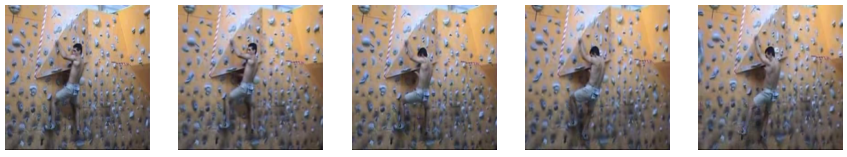
\includegraphics[width=\textwidth]{./images/rockclimbing}\hfill

\caption{Model je predvidio točan razred "RockClimbingIndoor" sa izlazom modela 0.9987.}
\label{fig:rockclimbing}
\end{subfigure}
\begin{subfigure}{\textwidth}

\centering
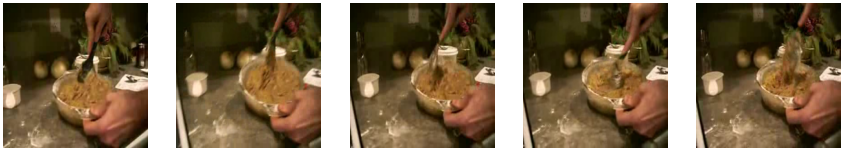
\includegraphics[width=\textwidth]{./images/mixing}\hfill

\caption{Model je predvidio točan razred "Mixing" sa izlazom modela 0.4043. Drugi najveći izlaz je za razred "BlowingCandles" sa vrijednosti 0.375.}
\label{fig:mixing}
\end{subfigure}
\begin{subfigure}{\textwidth}

\centering
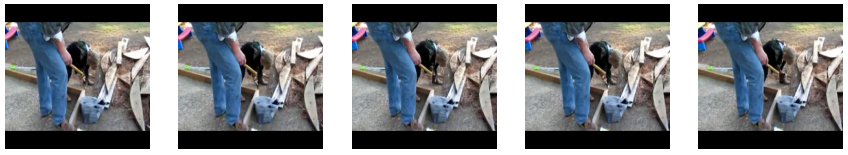
\includegraphics[width=\textwidth]{./images/hammering2}\hfill

\caption{Model je predvidio točan razred "Hammering" sa izlazom modela 0.3520.}
\label{fig:hammering2}
\end{subfigure}
\caption{Prikaz nekoliko podataka iz testnog skupa na kojima model ostvaruje dobre rezultate.}
\end{figure}
\newpage
 Na slici koja prikazuje video prikaz ljuljanja na ljuljački \ref{fig:swing} vidimo da je model pogrešno procijenio da je na videu prikazana šetnja psa. Na videu se stvarno nalazi pas i osoba što je specifično za radnju šetnje psa, dok se osoba na ljuljački jako brzo pomiče što otežava prepoznavanje točne radnje. Za video prikazan slikom \ref{fig:hammering} model pogrešno tvrdi da je na videu prikazano šišanje. Drugi izlaz modela je sušenje kose. Model smatra da je okolina u kojem se odvija radnja udaranja čekićem specifičnija za šišanje ili sušenje kose. Model ima problema sa raspoznavanjem između kriket-kuglanja i kriketa kao što uočavamo na slici \ref{fig:cricket}. Analizom podataka iz skupa smo ustanovili da su radnje obično snimane u sličnim okolnostima i ne razlikuju se znatno. 
\begin{figure}[htp]
\begin{subfigure}{\textwidth}

\centering
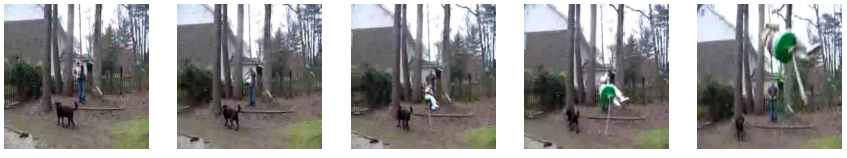
\includegraphics[width=\textwidth]{./images/swing}\hfill

\caption{Model je pogrešno predvidio "WalkingWithDog" sa izlazom modela 0.5115, stvarni razred je "Swing".}
\label{fig:swing}
\end{subfigure}

\begin{subfigure}{\textwidth}

\centering
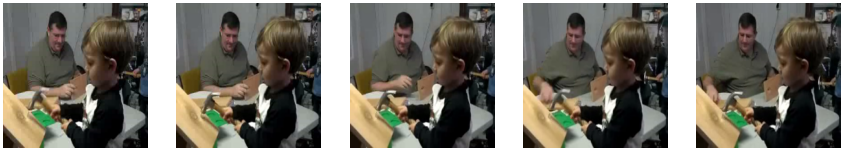
\includegraphics[width=\textwidth]{./images/hammering}\hfill

\caption{Model je predvidio razred "Haircut" sa izlazom modela 0.3753. Drugi izlaz sa najveći izlaz je za razred "BlowDryHair" sa vrijednosti 0.2365. Točan razred je "Hammering".}
\label{fig:hammering}
\end{subfigure}

\begin{subfigure}{\textwidth}

\centering
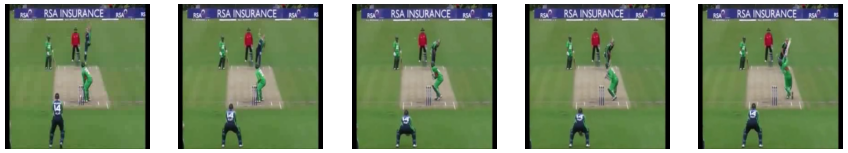
\includegraphics[width=\textwidth]{./images/cricketshot}\hfill

\caption{Model je predvidio razred "CricketBowling" sa izlazom modela 0.9991 dok je točan razred "CricketShot".}
\label{fig:cricket}
\end{subfigure}
\caption{Prikaz nekoliko podataka iz testnog skupa na kojima model ne ostvaruje dobre rezultate.}
\end{figure}

\chapter{Zaključak}
Računalni vid obiluje nerješenim problemima kojima se sve češće pristupa korištenjem metoda dubokog učenja. Zahvaljujući rapidnom razvoju hardvera i tehnika koje se koriste u dubokom učenju, takve metode pokazuju sve bolje rezultate. U ponekim problemima takvi modeli čak i nadmašuju performanse čovjeka. Na Imagenet problemu je ljudska top-5 pogreška klasifikacije bila $5.1\%$, dok su već modeli iz 2017. ostvarivali top-5 pogrešku klasifikacije od $3.57\%$ \cite{humans}.
\par
U sklopu ovog rada smo se upoznali sa kovolucijskim modelima za klasifikaciju videa. Upoznalni smo koji skupovi postoje za klasifikaciju videa i pobliže smo se upoznali sa skupom UCF-101 na kojem smo provodili eksperimente. Naučili smo koristiti Keras programski okvir za strojno učenje. Napravili smo sustav za klasifikaciju videa pomoću navedenog programskog okvira. Izdvojili smo dvije konkretne arhitekture s kojima smo se detaljno upoznali i koje smo u konačnici implementirali. Objasnili smo ključne pojmove koji se kriju iza učenja takvih modela. Objasnili smo kako rade i kako se konstruiraju konvolucijski modeli. Ukratko smo opisali kralježničke arhitekture koje smo koristili u sklopu naših eksperimenata. Predstavili smo dvije mogućnosti kako pristupiti videu kao podatku za učenje, pri čemu smo opisali svoja iskustva sa navedenim mogućnostima i dali preporuke za korištenje ovisno o računalnim resursima dostupnim prilikom učenja.
\par
Sa modelima sa sažimajućim značajkama smo ostvarili maksimalni rezultat od $71.73\%$ sa MobileNetV2 kralježničkom arhitekturom. Sa ResNet18 i MobileNet arhitekturama smo ostvarili nešto lošiji rezultat, što smo i očekivali jer MobileNetV2 i na problemima poput klasifikacije slika ostvaruje bolji rezultat. Sa SlowFast arhitekturom smo postigli rezultat od $42.95\%$ točnosti klasifikacije na testnom skupu. Očekivali smo da će rezultat SlowFast arhitekture nadmašiti rezultate ostvarene sa modelima sa sažimajućim značajkama. Smatramo da je rezultat lošiji od rezultata ostvarenog sa modelima sa sažimajućim značajkama zbog greške u implementaciji ili zbog lošeg izbora hiperparametara. Proveli smo eksperiment sa 10 okvira uzorkovanih iz jednog videa i uvjerili se da modeli ostvaruju lošiji rezultat u odnosu na ostale modele koji koriste 32 okvira iz videa. Rezultat je očekivan jer modeli koji na ulazu primaju manje okvira iz videa vide potencijalno manje konteksta videa.
\par
U budućim eksperimentima bi svakako bilo poželjno ispitati kako bi se ponašali modeli uz uvođenje optičkog toka u modele. U okviru modela sa sažimajućim značajkama bi se mogli provesti eksperimenti sa ostalim načinima sažimanja. Zanimljivo bi bilo vidjeti i kako bi se modeli ponašali na većim skupovima poput skupa Kinetics-400. 
\bibliography{literatura}
\bibliographystyle{fer}

\begin{sazetak}
Klasifikacija videa neriješen je problem računalnog videa s mnogim zanimljivim primjenama. U posljednje vrijeme najbolji rezultati u tom području postižu se pristupima temeljenim na dubokim konvolucijskim modelima. Za ovaj rad posebno su zanimljivi nadzirani pristupi gdje je svaki video označen razredom radnje koju video predstavlja. U okviru rada proučio sam postojeće pristupe klasifikaciji videa. Objasnio sam teorijsku podlogu bitnu za razumijevanje eksperimenata koji se provode. Izrađena implementacija modela temelji se na radnom okviru Keras. Izgradio sam dvije konkretne arhitekture za klasifikaciju videa. Opisao sam i arhitekture na kojima se arhitekture od interesa baziraju. Prikazao sam i ocjenjenio ostvarene rezultate i predložio pravce za budući razvoj.
\kljucnerijeci{duboko učenje, klasifikacija videa, konvolucijski modeli za klasifikaciju videa, Keras, UCF-101, SlowFast, sažimanje značajki}
\end{sazetak}
\newpage
% TODO: Navedite naslov na engleskom jeziku.
\engtitle{Convolutional models for video classification}
\begin{abstract}
Video classification is an unsolved problem of computer vision with many interesting applications. Lately, best results in that area are obtained using approaches based on deep convolutional models. This thesis considers supervised approaches where every video is labeled with class of action the video represents. I examined existing approaches to video classification which were interesting for this paper. I explained the theory necessary for undestanding of the experiments. Model impementation is based on Keras framework. I have built two distinct architectures for video classification. Additionaly, I have explained the architectures on which the architectures of interest are based. I reported the results and compaired them with results from literature and listed possible improvements and directions for future work.

\keywords{deep learning, video classification, convolutional models for video classification, Keras, UCF-101, SlowFast, feature-pooling}
\end{abstract}

\end{document}
